%
% assembly.tex
%
% Copyright The SLCam Contributors.
%
% SLCam Documentation
%
% This work is licensed under the Creative Commons Attribution-ShareAlike 4.0
% International License. To view a copy of this license,
% visit http://creativecommons.org/licenses/by-sa/4.0/.
%

%
% \brief Assembly instructions.
%
% \author Gabriel Mariano Marcelino <gabriel.mm8@gmail.com>
%
% \version 0.2.0
%
% \date 2024/04/14
%


\chapter{Assembly instructions} \label{anx:assembly}

This appendix presents the assembly instructions of the SLCam module.

\section{List of parts}

\begin{itemize}
    \item Controller board
    \item Image sensor board
    \item Metal case
    \item Screw \textcolor{red}{XXX}
    \item \textcolor{red}{TBC}
\end{itemize}

\begin{figure}[!ht]
    \begin{center}
        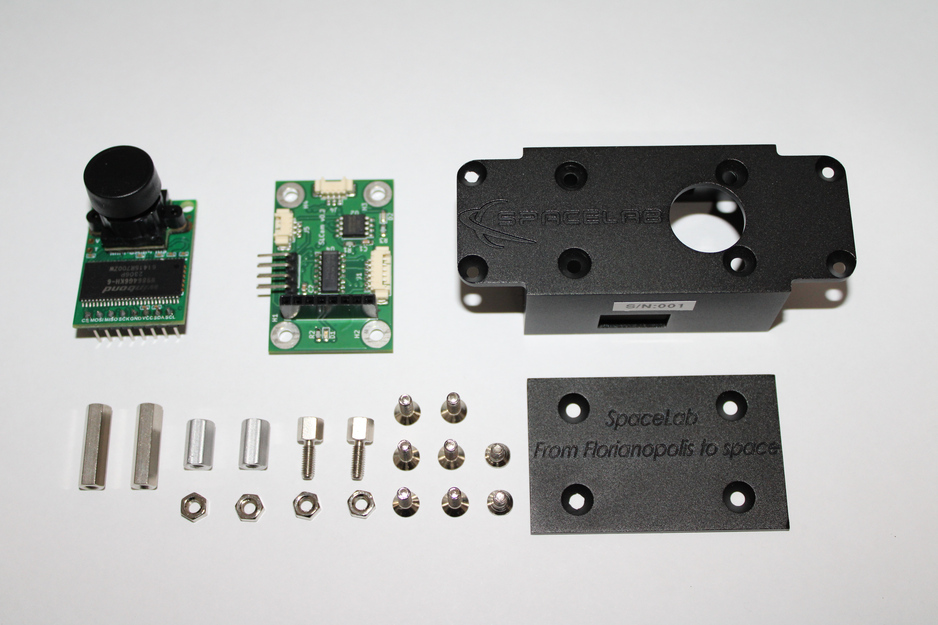
\includegraphics[width=\textwidth]{figures/assembly-parts.jpg}
        \caption{Parts of the SLCam.}
        \label{fig:assembly-parts}
    \end{center}
\end{figure}

\section{Assembly steps}

\begin{figure}[!ht]
    \begin{center}
        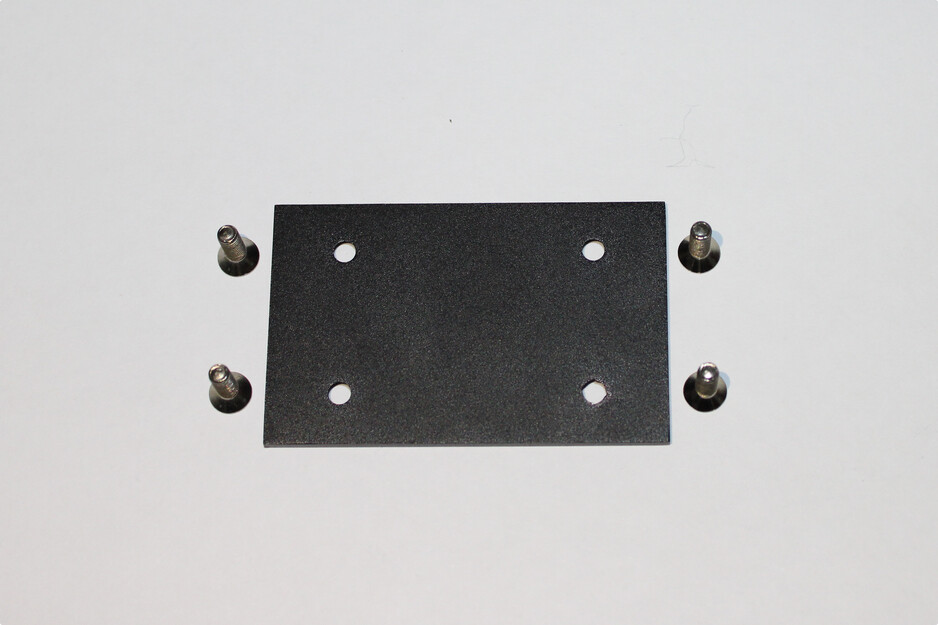
\includegraphics[width=\textwidth]{figures/step1.jpg}
        \caption{Step 1.}
        \label{fig:assembly-step-1}
    \end{center}
\end{figure}

\begin{figure}[!ht]
    \begin{center}
        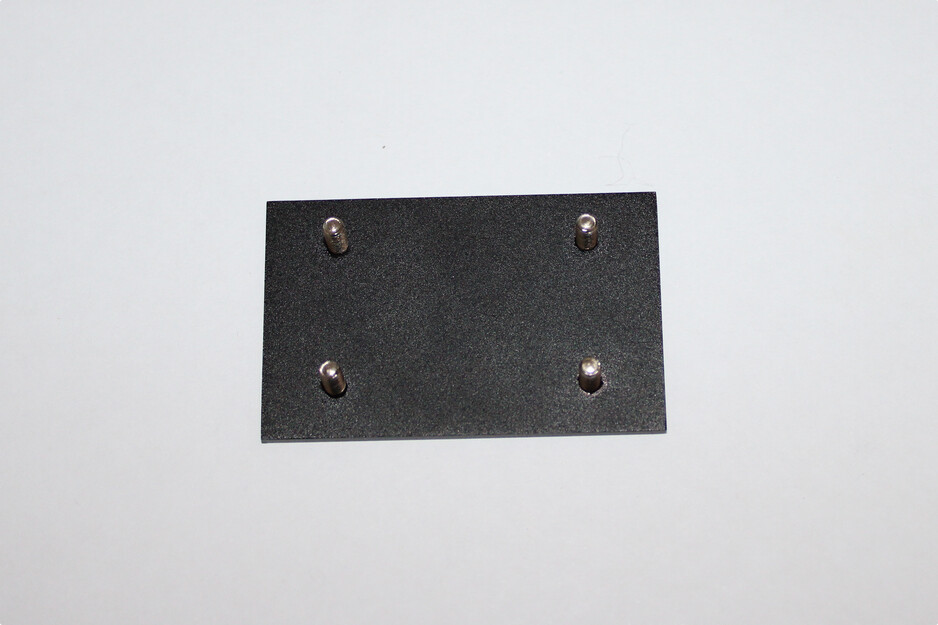
\includegraphics[width=\textwidth]{figures/step2.jpg}
        \caption{Step 2.}
        \label{fig:assembly-step-2}
    \end{center}
\end{figure}

\begin{figure}[!ht]
    \begin{center}
        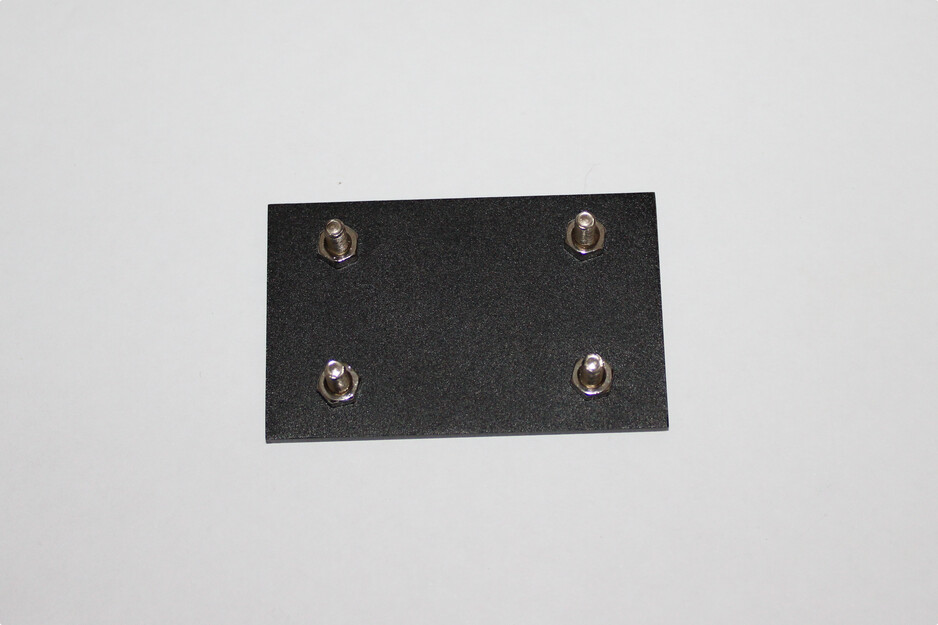
\includegraphics[width=\textwidth]{figures/step3.jpg}
        \caption{Step 3.}
        \label{fig:assembly-step-3}
    \end{center}
\end{figure}

\begin{figure}[!ht]
    \begin{center}
        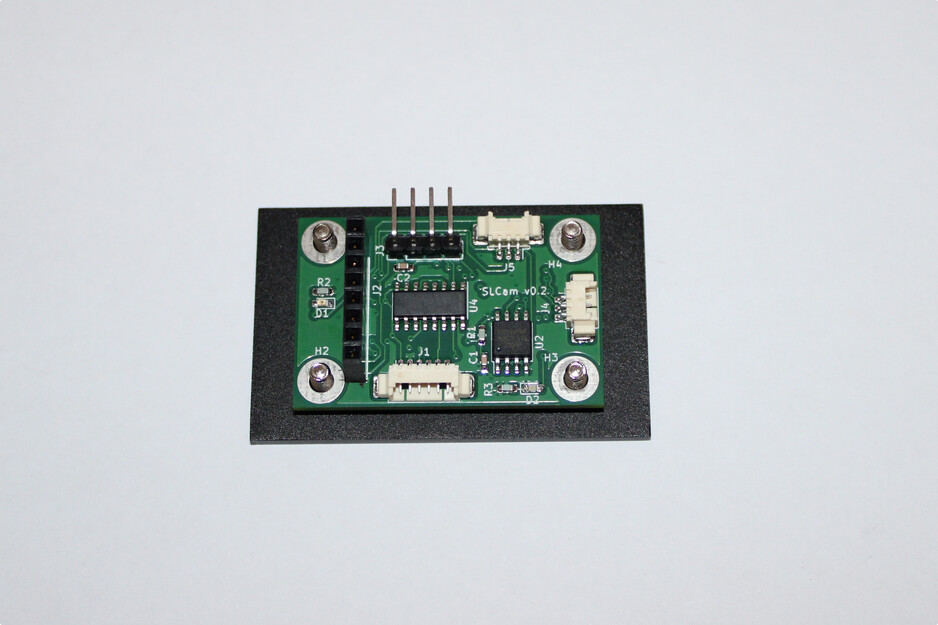
\includegraphics[width=\textwidth]{figures/step4.jpg}
        \caption{Step 4.}
        \label{fig:assembly-step-4}
    \end{center}
\end{figure}

\begin{figure}[!ht]
    \begin{center}
        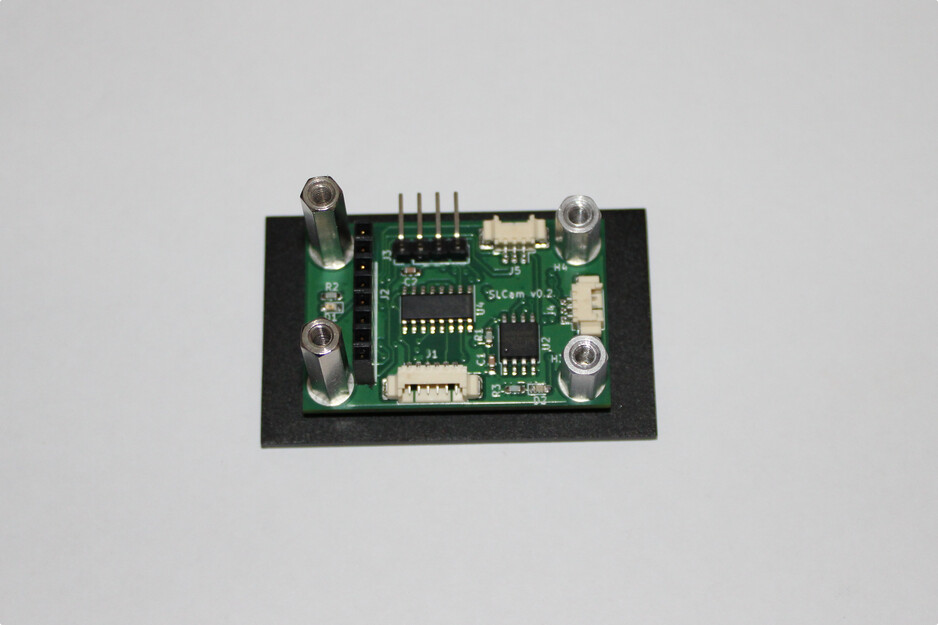
\includegraphics[width=\textwidth]{figures/step5.jpg}
        \caption{Step 5.}
        \label{fig:assembly-step-5}
    \end{center}
\end{figure}

\begin{figure}[!ht]
    \begin{center}
        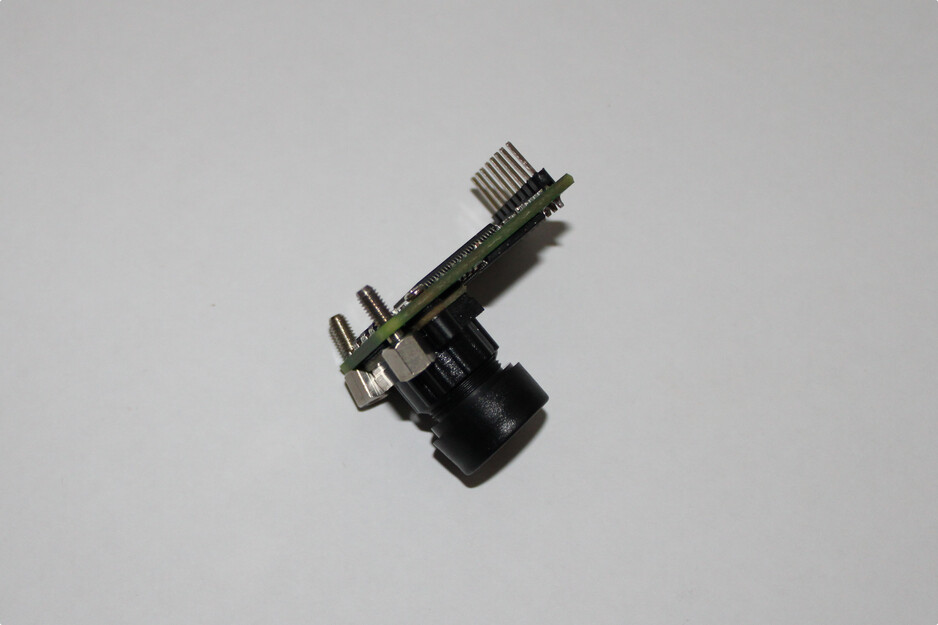
\includegraphics[width=\textwidth]{figures/step6.jpg}
        \caption{Step 6.}
        \label{fig:assembly-step-6}
    \end{center}
\end{figure}

\begin{figure}[!ht]
    \begin{center}
        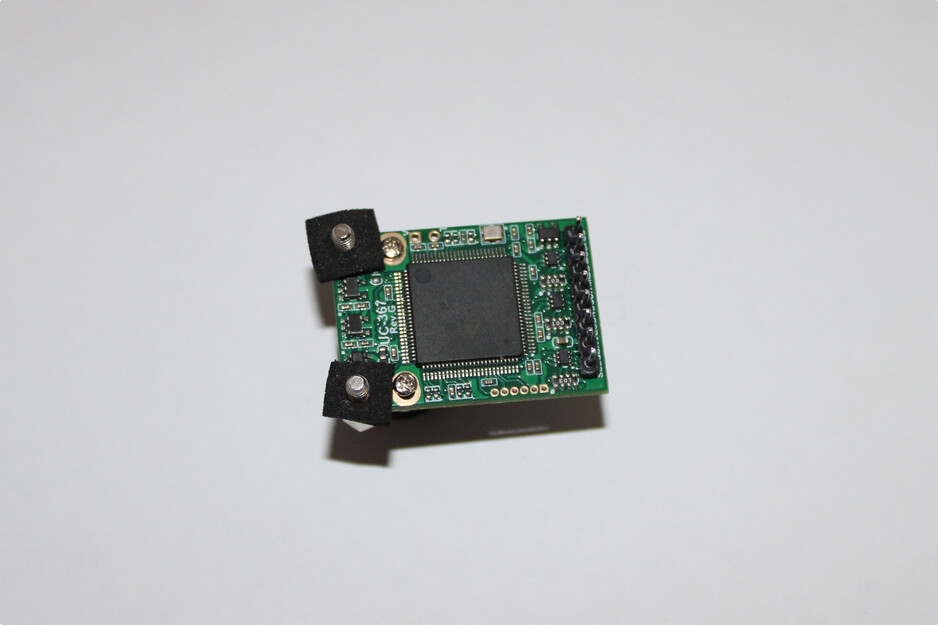
\includegraphics[width=\textwidth]{figures/step7.jpg}
        \caption{Step 7.}
        \label{fig:assembly-step-7}
    \end{center}
\end{figure}

\begin{figure}[!ht]
    \begin{center}
        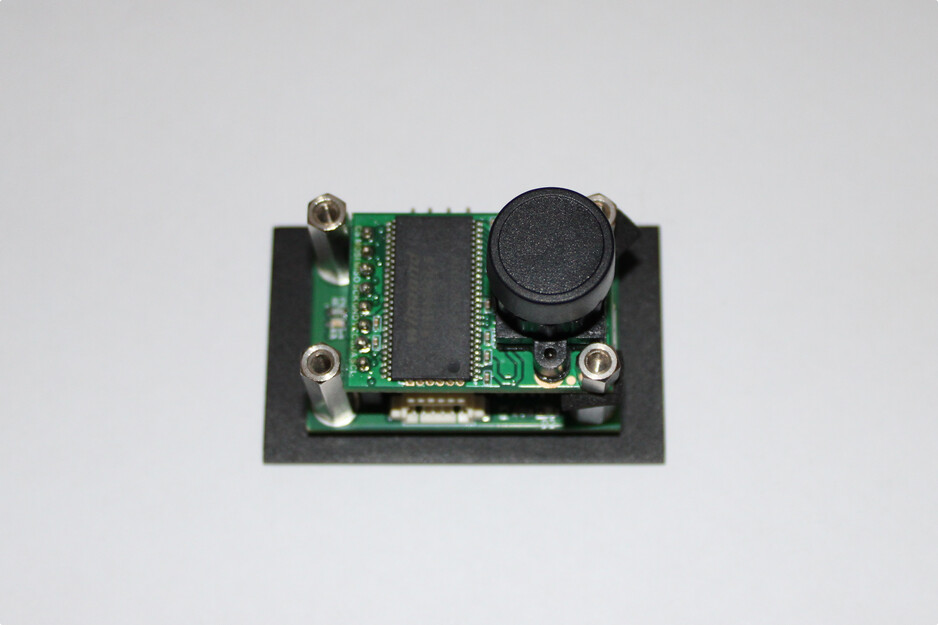
\includegraphics[width=\textwidth]{figures/step8.jpg}
        \caption{Step 8.}
        \label{fig:assembly-step-8}
    \end{center}
\end{figure}

\begin{figure}[!ht]
    \begin{center}
        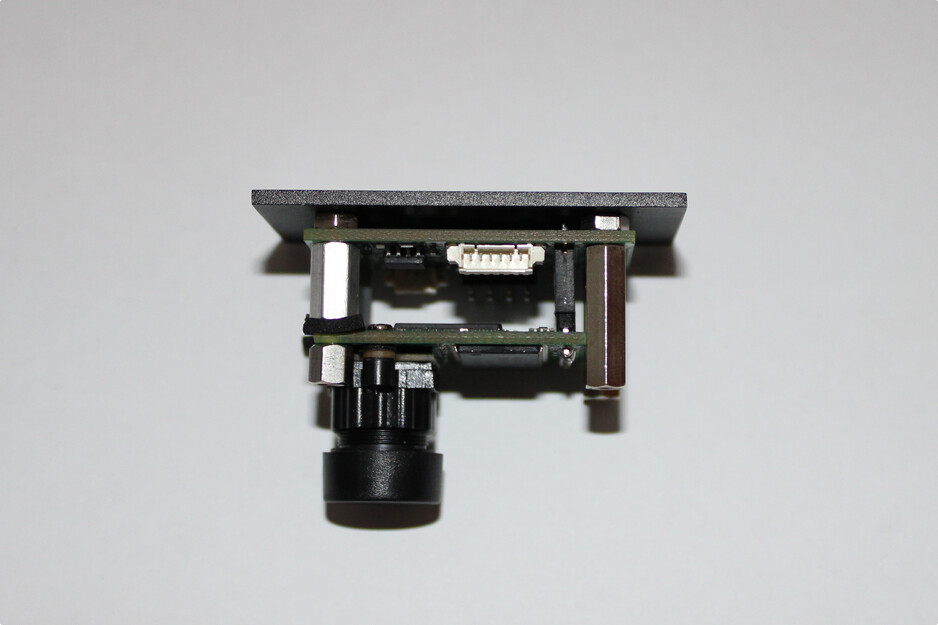
\includegraphics[width=\textwidth]{figures/step9.jpg}
        \caption{Step 9.}
        \label{fig:assembly-step-9}
    \end{center}
\end{figure}

\begin{figure}[!ht]
    \begin{center}
        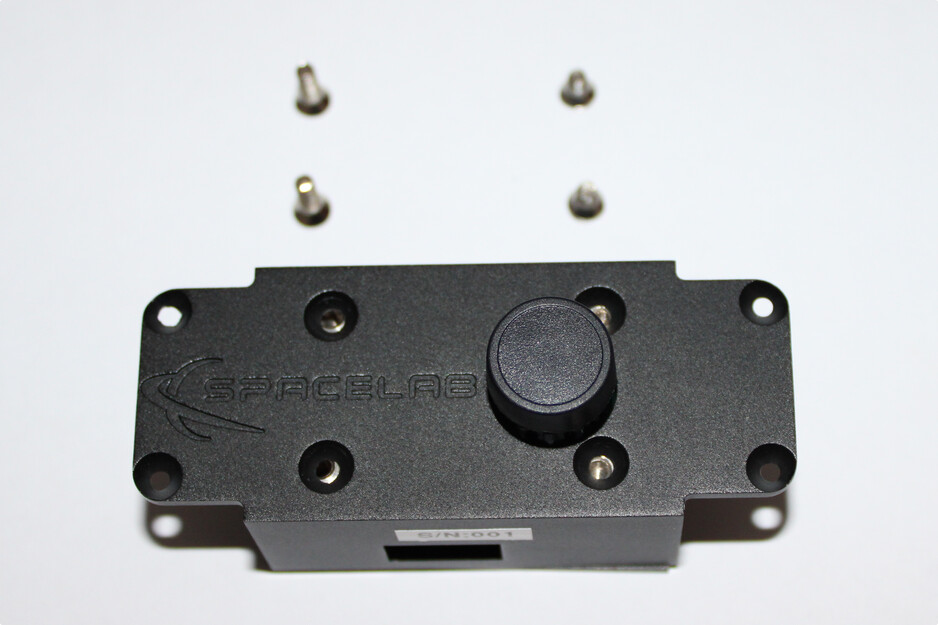
\includegraphics[width=\textwidth]{figures/step10.jpg}
        \caption{Step 10.}
        \label{fig:assembly-step-10}
    \end{center}
\end{figure}

\begin{figure}[!ht]
    \begin{center}
        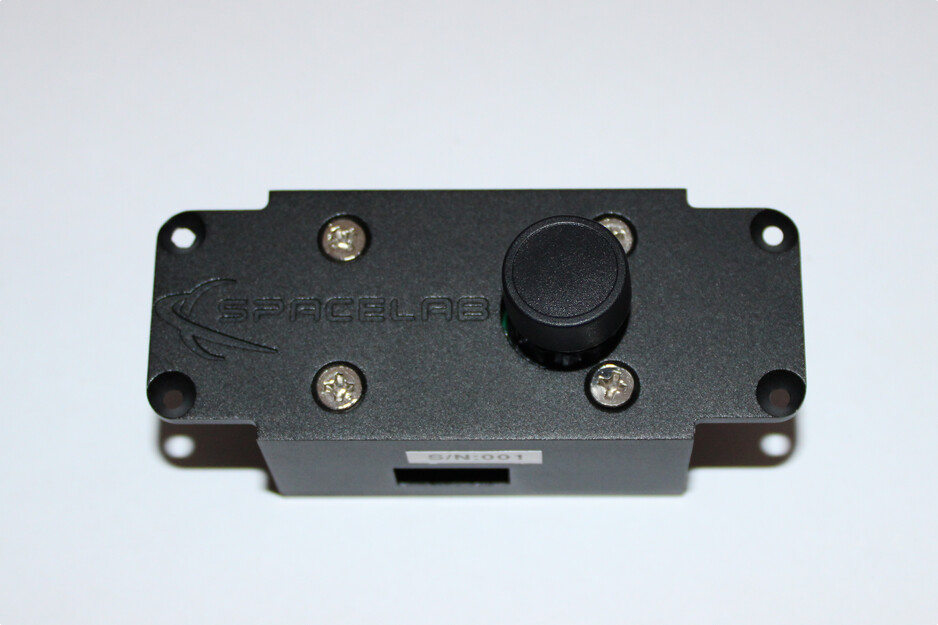
\includegraphics[width=\textwidth]{figures/step11.jpg}
        \caption{Step 11.}
        \label{fig:assembly-step-11}
    \end{center}
\end{figure}